

% LaTeX file for Chapter 02


\chapter{Methods} 

In this section I will explain the necessary background needed to understand the TRAM-DAGs. Once the framework of tram dags is explained, I will present how the experiments of the simulation, the application on real data and the ITE estimation are conducted.


The goal of TRAM-DAGs is to estimate the structural equations according to the causal order in a given DAG in a flexible and possibly still interpretable way in order to sample observational and interventional distributions and to make counterfactual statements. The estimation requires data and a DAG that describes the causal structure. It must be assumed that there are no hidden confounders. TRAM-DAGs estimate for each variable $X_i$ a transformation function $Z_i = h_i(X_i \mid pa(X_i))$, where $Z_i$ is the noise value and $pa(X_i)$ are the causal parents of $X_i$. The important part here is that we can rearrange this equation to $X_i = h_i^{-1}(Z_i \mid pa(x_i))$ to get to the structural equation. The transformation functions $h$ are monotonically increasing functions that are a representation of the conditional distribution of $X_i$ on a latent scale. They are based on the idea of transformation models as introduced by \citet{hothorn2014} but were extended to deep trams by \citet{sick2020}. In the following sections I review the most important ideas of these methods as they are the essential components of TRAM-DAGs.

\section{Transformation Models}


Transformation models are a flexible distributional regression method for various data types. They can be for example specified as ordinary linear regression, logistic regression or proportional odds logistic regression. But Transformation models further allow to model conditional outcome distributions that do not even need to belong to a known distribution family of distributions by model it in parts flexibly. This reduces the strength of the assumptions that have to be made.

The basic form of transformation models can be described by 

\begin{equation}
F(y|\mathbf{x}) = F_Z(h(y \mid \mathbf{x}) =  F_Z(h_I(y) - \mathbf{x}^\top \boldsymbol{\beta})
\end{equation}

, where $F(y|\mathbf{x})$ is the conditional cumulative distribution function of the outcome variable $Y$ given the predictors $\mathbf{x}$. $h(y \mid \mathbf{x})$ is a transformation function that maps the outcome variable $y$ onto the latent scale of $Z$. $F_Z$ is the cumulative distribution function of a latent variable $Z$, the so-called inverse-link function that maps $h(y \mid \mathbf{x})$ to probabilities. In this basic version, the transformation function can be split into an intercept part $h_I(y)$ and a linear shift part $\mathbf{x}^\top \boldsymbol{\beta}$, where the vector $\mathbf{x}$ are the predictors and $\boldsymbol{\beta}$ are the corresponding coefficients.

If the latent distribution $Z$ is chosen to be the standard logistic distribution, then the coefficient $\beta_i$ can be interpreted as log-odds ratios when increasing the predictor $x_i$ by one unit, holding all other predictors unchanged. This means that an increase of one unit in the predictor $x_i$ leads to an increase of the log-odds of the outcome $Y$ by $\boldsymbol{\beta}$. The additive shift of the transformation function means a linear shift on the latent scale (herer log-odds). The following transformation to probabilities by $F_Z$ potentially leads to a non-linear change in the conditional outcome distribution on the original scale. This means not only is the distribution shifted, also its shape can change to some degree based on the covariates. More details about the choice of the latent distribution and the interpretation of the coefficients are provided in the appendix XXX. 


For a continuous outcome $Y$ the intercept $h_I$ is represented by a bernstein polynomial, which is a flexible and monotonically increasing function

\begin{equation}
h_I(y) = \frac{1}{M + 1} \sum_{k=0}^{M} \vartheta_k \, \text{B}_{k, M}(y)
\end{equation}

, where $\vartheta_k$ are the coefficients of the bernstein polynomial and $\text{B}_{k, M}(y)$ are the Bernstein basis polynomials. More details about the technical implementation of the bernstein polynomial in the context of TRAM-DAGs is given in the appendix XXX.

For a discrete outcome $Y$ the intercept $h_I$ is represented by cut-points, which are the thresholds that separate the different levels of the outcome. For example, for a binary outcome $Y$ there is one cut-point and for an ordinal outcome with $K$ levels there are $K-1$ cut-points. The transformation model is given by

\begin{equation}
P(Y \leq y_k \mid \mathbf{X} = \mathbf{x}) = F_Z(\vartheta_k + \mathbf{x}^\top \boldsymbol{\beta}), \quad k = 1, 2, \ldots, K - 1
\end{equation}


A visual representation for a continuous and discrete (ordinal) outcome is provided in Figure~\ref{fig:tram_cont_ord}.


% include image /img/tram_cont_ord.png
\begin{figure}[H]
\centering
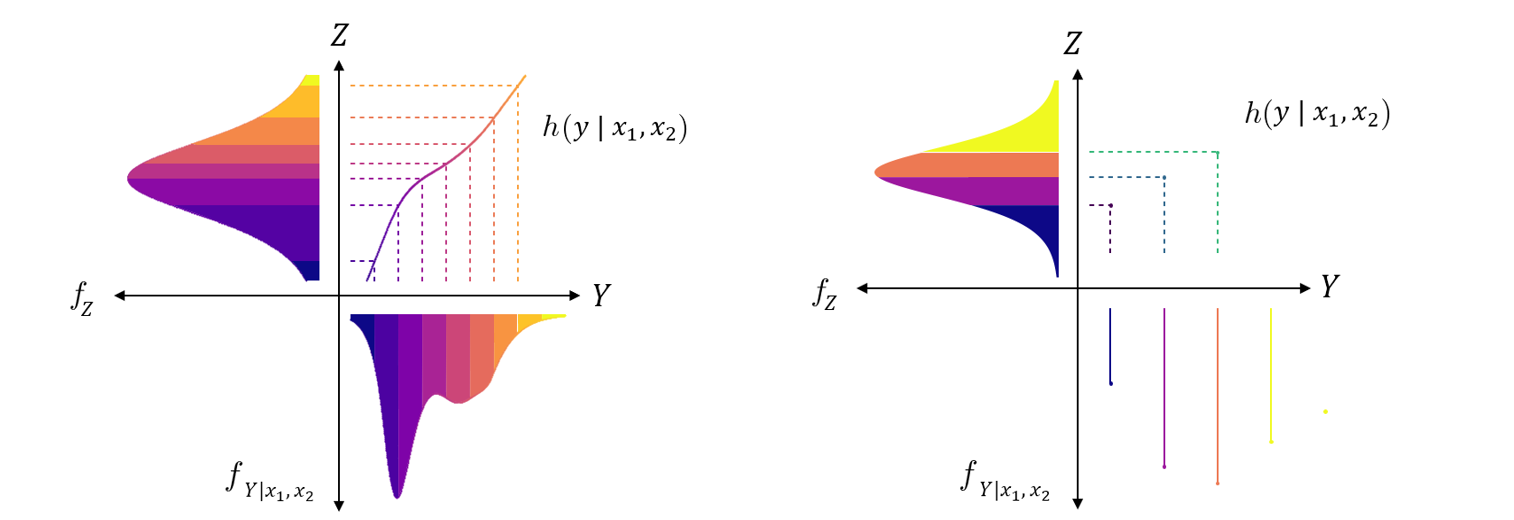
\includegraphics[width=1\textwidth]{img/tram_cont_ord.png}
\caption{\textbf{Left:} Example of a transformation model for a continuous outcome $Y$ with a smooth transformation function. \textbf{Right:} Example of a transformation model for an ordinal outcome $Y$ with 5 levels. The transformation function consists of cut-points that separate the probabilities for the levels of the outcome.
In both cases the latent distribution $Z$ is the standard logistic and the predictors $\mathbf{x}$ induce a linear (vertical) shift of the transformation function.}
\label{fig:tram_cont_ord}
\end{figure}


For the remainder of this thesis, I rely on the idea of these transformation models to model the conditional distribution functions represented by the transformation functions of the respective variables. The standard logistic distribution is used as $F_Z$, which results in a logistic transformation model.


\section{Deep TRAMs}

The transformation models as discussed before were extended to deep TRAMs using neural networks. The goal is to get a parametrized transformation function by training a modular neural network and thereby minimizing the NLL. This minimization is done with Deep learning optimization methods.

\begin{figure}[H]
\centering
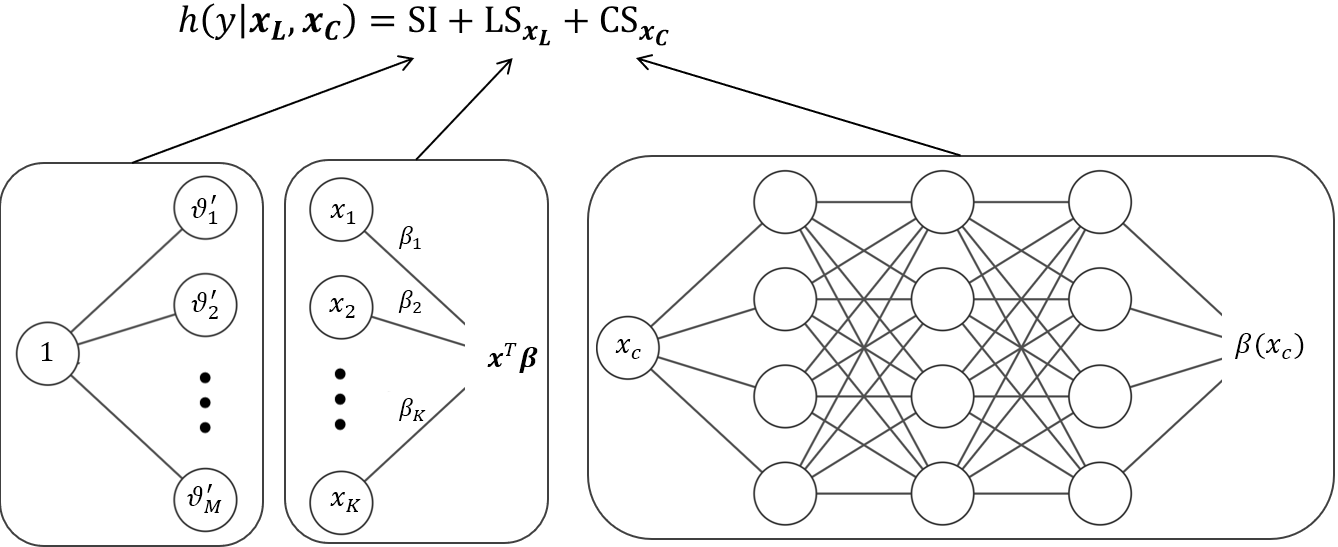
\includegraphics[width=0.9\textwidth]{img/deep_tram.png}
\caption{Modular deep transformation model. The transformation function $h(y \mid \mathbf{x})$ is constructed by the outputs of three neural networks.}
\label{fig:deep_tram}
\end{figure}

So on the slides you can see again the transformation function for the outcome Y that depends on the covariates X. Here, XL should stand for the predictors that shift the transformation function in a linear manner (as in the examples on the previous slides) and XC stands for Predictors that have a non linear influence. And the cool thing here is that these Complex Predictors could also include something like an Image.

The first part of the transformation function is a Simple intercept which is responsible for the baseline shape of the distribution. This intercept is constructed by a neural network, that takes no predictors as input and just outputs the parameters for the Bernstein polynomial or for the cut points in the discrete case. If we wanted to allow for more flexibility, we could give a predictor as input instead of just a constant, but in this presentation I will only show the simple case.

Next there is a Linear Shift which is basically a linear combination of the linear predictors. We can obtain this by creating another neural network with no hidden layers taking only the predictors as input and producing the linear shift as output.

Finally there is the complex shift which we obtain by giving the complex predictors into a neural network with some hidden layers and getting a single number as output.

The Neural Network training happens iteratively by starting with a (random) parameter configuration and then using the outputted intercepts and shift to calculate the loss, which is the negative log likelihood of our transformation model. To improve the loss, the parameters are then slightly adjusted by the adam optimizer. Then the process is repeated until the parameter estimates converge. So this means we are optimizing the negative log likelihood of the logistic transformation model, which represents the conditional distribution function of our outcome variable. 

The nice thing of these deep transformation models is that we can specify, whether we want a linear shift bx or a complex shift b(x) or even a complex intercept and thereby controlling the flexibility.


\textbf{TRAM-DAGs}

And here you can see how this looks in our case, where we apply these deep transformation models in a causal setting. So we assume a pre-specified DAG which defines the Causal dependence. And then we model each node by a transformation model that is conditional on its parents.

In this Example dag we have 3 variables:

X1 is continuous and a source node, meaning it has no parents that it depends on, hence the transformation function h only represents the intercept.

Then X2 depends on X1, so this means that the transformation function changes with X1. In what way the transformation function is allowed to change, has to be specified. This could either be a linear or complex shift or even a complex intercept.

And finally there is the ordinal variable X3 which has 4 levels. The Transformation function consists of 3 cut points that depend on X1 and X2. These cut-points represent the Probabilities of the 4 levels of X3.

Choice of link function does not matter if fully flexible (CI) but it puts some assumptions if not fully flexible. Same as in the sense of the SCM where the choice of the Noise distribution can matter (depending on how flexible the equations are).


Ok so lets make a simulation example and put this all together.

First of all we have observational data that follows a pre-defined DAG without hidden confounders. In practice such a dag can be defined by expert knowledge or by some sort of structure finding algorithm.

Then we want to estimate the conditional distribution function of each variable so that we can sample from the distributions and make causal queries.

So in this example we assume the same dag as on the previous slide with the 3 variables. X1 and X2 are continuous and X3 is ordinal. Now we also specify how these variables are related. So X1 is the source node. X2 depends on X1 through a linear shift and X3 depends on X1 by a linear shift and on X2 by a complex shift.


This model structure can also be presented by an adjacency matrix where the rows indicate the source of effect and the columns are the target of the effect. In our algorithm we use this Meta-adjacency matrix to control the information flow.





\textbf{Construct Modular Neural network}

Now we set up a modular neural network which produces the components of the transformation functions as outputs. The Adjacency Matrix thereby controls the information flow. Here you also can see the number of parameters. In total there are 281 Parameters in this model, but not all of them are used I will not get into the details here. On the right side you can also see the neural network that produces the complex shift from X2 to X3. We chose to model it by 4 hidden layers with 2 nodes each. That should allow for high enough flexibility.

Finally the outputs of the different Neural network parts are combined to the transformation functions for each node, from which we then derive the negative log likelihood.

Optimizers and hyperparameters etc

Adam, Batchnormalization, activation functions (relu, sigmoid)
Impact of Scaling (maybe in Appendix)
Neural network works best if inputs are scaled. Proof that we can do that, it just changes the interpretation. For structure finding algorithms, this might be problematic, because increasing variance along the causal order would be destroyed. (why, how, interpretation change etc. check meeting notes 22.04.2025)

Different Intercepts, and Shifts

and show, describe how the transformation function and hence the conditional distribution will change in each scenario. Also show in detail how the neural networks would be set up, how the information flow is controlled and what kind of outputs are produced and how they further have to be transformed.

Describe interpretation quickly and refer to formal proof in the Appendix.
%  for interpretation see pearl book 2009 p. 366. the key is to say leaving all other variables "untouched" and not "constant". he also talks about the connection to the do-operator.

Fitting Betas Interpretable

The two parameters for our linear shift terms are plotted here. We can see that they converge quickly to the same values as we used in the DGP. We can interpret these parameters as log-odds ratios if changing the value of the parent by one unit.

Intercepts

Show the Discrete case with just cutpints (only K-1 parameters of outputs are used)
Show the continuous case where the outputs are transformed to monotonically increasing betas for the bernstein polynomial. Also describe Bernstein polynomial construction in detail with scaling and linear extrapolation.

Here I plotted the intercepts of the 3 transformation functions. They also resemble the DGP very nicely.


Linear and complex shifts

Here in the first two plots we can see the linear shifts. And in the right plot we have the complex shift of X2 on X3. The estimated shifts match quite well with the DGP.

Complex shift (Interaction example) to show what is also possible

Here I just want to make a short input from another example. So there the true model was that of a logistic regression with the binary outcome Y and 3 predictors. The binary treatment T and the two continuous predictors X1 and X2. There was also an interaction effect assumed between treatment and X1. So this basically means that the effect of X1 on the outcome is different for the two treatment groups.

And here we can show that our TRAM-DAG specified by a complex shift of T and X1 can also capture this interaction effect quite well.


Loss function

And this is how the negative log likelihood looks like for a continuous outcome. It is derived from the CDF based on the logistic transformation model. A special thing here is that the outcome variable has to be scaled to the range between 0 and 1 first, and this scaling also has to be considered when calculating the NLL. But I will not go through this now.
For final Loss, the individual losses of the nodes are added together. (only in R framework, in Python they are fitted individually?)


NN Training

Now we have everything in place to train the neural network. Here I run the model for 400 Epochs (which means that the model has seen each sample 400 times). On the right you can see the loss of the training set and also the validation loss as comparison. The NLL quickly dropped to around 1.1 and then didnt change much anymore, which indicates that the parameter estimates have probably converged to a good state.


\textbf{discrete predictors}

\textbf{sampling from the tram dag}
Each variable Xi in the DAG can be described by a structural equation Xi = f(Zi, pa(Xi)). For a continous outvome x1, in TRAM-DAGs this structural equation is the inverse of the conditional transformation function Xi = h-1(Zi | pa(Xi)). for a discrete outcome it is defined as... show sampling.

Refer back to the SCM, that we basically can obtain the structural equations from our model. Okay so now we have estimates for the conditional transformation functions of our 3 variables. To generate a sample for a node, we first sample a random value from the latent distribution. In our case from the standard logistic. We denote this sample as Z.

Next we want to determine the value of the Node X. If X is continuous, we can apply the inverse of the transformation function evaluated at Z to find X. If X is ordinal, we just select the corresponding category that belongs to the next bigger cut-point.

If we want to make a do-intervention, we just fix a node at the desired value.


\textbf{counterfactuals}

Describe how to do it, limitations etc.

see pearl book causality: 1.4.4 Counterfactuals in Functional Models


\textbf{ITE how it is applied in our model?}

RCTs only measure the average treatment effect. There will be patients who respond better or worse to the treatment because patient specific characteristcs. In personalized medicine however, the aim is to find the optimal treatment for a specific individual. Such a measure that can help in decision making is the ITE.

Rubins potential outcomes framework.


Maybe it is the methods section. Here however, we give a couple hints.
Note that you can wisely use \rr{preamble}-chunks. Minimal, is likely: 

\bigskip

\hrule
\begin{knitrout}
\definecolor{shadecolor}{rgb}{0.969, 0.969, 0.969}\color{fgcolor}\begin{kframe}
\begin{verbatim}
library(knitr) 
opts_chunk$set( 
    fig.path='figure/ch02_fig',    
    self.contained=FALSE,
    cache=TRUE
) 
\end{verbatim}
\end{kframe}
\end{knitrout}
\hrule

\bigskip

Defining figure options is very helpful:

 
\bigskip


\hrule
\begin{knitrout}
\definecolor{shadecolor}{rgb}{0.969, 0.969, 0.969}\color{fgcolor}\begin{kframe}
\begin{verbatim}
library(knitr)
opts_chunk$set(fig.path='figure/ch02_fig',
               echo=TRUE, message=FALSE,
               fig.width=8, fig.height=2.5,  
               out.width='\\textwidth-3cm',
               message=FALSE, fig.align='center',
               background="gray98", tidy=FALSE, #tidy.opts=list(width.cutoff=60),
               cache=TRUE
) 
options(width=74)
\end{verbatim}
\end{kframe}
\end{knitrout}
\hrule

\bigskip 

This options are best placed in the main document at the beginning. Otherwise a \verb+cache=FALSE+ as knitr option is necessary to overrule a possible  \verb+cache=TRUE+ flag. 

\bigskip 

Notice how in Figure~\ref{f02:1} everything is properly scaled.   

\begin{figure}
\begin{knitrout}
\definecolor{shadecolor}{rgb}{0.98, 0.98, 0.98}\color{fgcolor}

{\centering 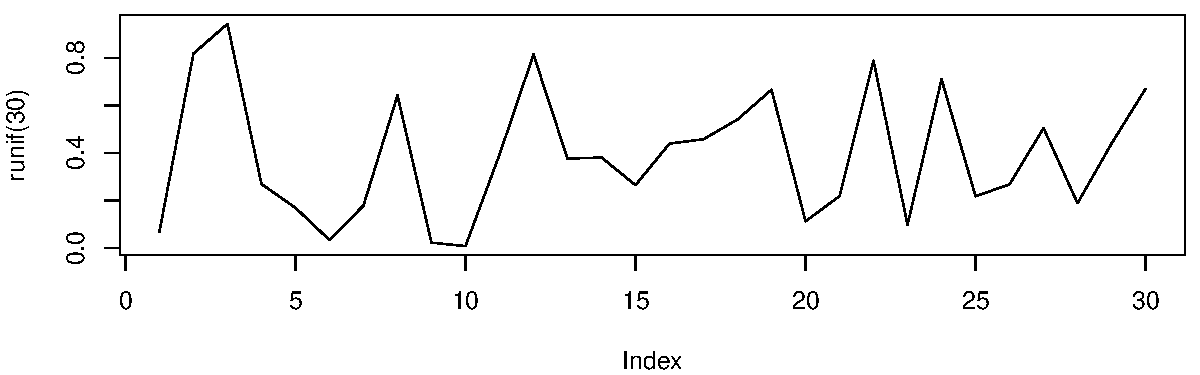
\includegraphics[width=\textwidth-3cm]{figure/ch02_figunnamed-chunk-3-1} 

}


\end{knitrout}
  \caption{Test figure to illustrate figure options used by knitr.}
  \label{f02:1}
\end{figure}


\section{Citations}

Recall the difference between \verb+\citet{}+ (e.g., \citet{Chu:Geor:99}), \verb+\citep{}+ (e.g., \citep{Chu:Geor:99}) and \verb+\citealp{}+ (e.g., \citealp{Chu:Geor:99}).
For simplicity, we include here all references in the file \verb+biblio.bib+ with the command \verb+\nocite{*}+.\nocite{*}

